\documentclass[12pt]{article}
\usepackage[a4paper,left=2.5cm,right=2.5cm,top=2.5cm,bottom=2.5cm]{geometry}
%\usepackage[margin=0.5in]{geometry}
\usepackage[utf8]{inputenc}
\usepackage{graphicx}
\usepackage{float}
\usepackage{multicol}
\usepackage{wrapfig}
\usepackage{multirow}
\usepackage{subcaption}
\graphicspath{ {images/} }




\begin{document}



\begin{titlepage}

\newcommand{\HRule}{\rule{\linewidth}{0.5mm}} % Defines a new command for the horizontal lines, change thickness hereru

\center % Center everything on the page
 
%----------------------------------------------------------------------------------------
%	HEADING SECTIONS
%----------------------------------------------------------------------------------------

\textsc{\LARGE Tata Institute of Fundamental Research}\\[1.5cm] 
%\textsc{\Large TIFR Graduate School Project Report, June 2018}\\[0.5cm] % Major heading such as course name
\textsc{\large Graduate School Project Report}\\[0.5cm] % Minor heading such as course title
\vspace{4cm}
%----------------------------------------------------------------------------------------
%	TITLE SECTION
%----------------------------------------------------------------------------------------

\HRule \\[0.4cm]
{ \huge \bfseries Comparison of CORSIKA hadronic interaction generators with GRAPES-3 data}\\[0.4cm] % Title of your document
\HRule \\[1.5cm]
 
%----------------------------------------------------------------------------------------
%	AUTHOR SECTION
%----------------------------------------------------------------------------------------

\vspace{4cm}

\begin{minipage}{0.4\textwidth}
\begin{flushleft} \large
\emph{Author:}\\
Mohit Saharan\\
DHEP, TIFR, Mumbai
% Your name
\end{flushleft}
\end{minipage}
~
\begin{minipage}{0.4\textwidth}
\begin{flushright} \large
\emph{Supervisor:} \\
Dr. Pravata K. Mohanty\\
DHEP, TIFR, Mumbai
\end{flushright}
\end{minipage}\\[2cm]

% If you don't want a supervisor, uncomment the two lines below and remove the section above
%\Large \emph{Author:}\\
%John \textsc{Smith}\\[3cm] % Your name

%----------------------------------------------------------------------------------------
%	DATE SECTION
%----------------------------------------------------------------------------------------

{\large \today}\\[2cm] % Date, change the \today to a set date if you want to be precise

%----------------------------------------------------------------------------------------
%	LOGO SECTION
%----------------------------------------------------------------------------------------

%\includegraphics{tifr_logo.png}\\[1cm] % Include a department/university logo - this will require the graphicx package
 
%----------------------------------------------------------------------------------------

\vfill % Fill the rest of the page with whitespace

\end{titlepage}
\pagebreak


\begin{abstract}
In GRAPES-3 experiment, hadronic interaction generators of CORSIKA simulation program are used to derive the composition and energy of primary cosmic rays (PCRs). The results are highly dependent on the assumptions taken by different type of  generators. This study compares the two generators from CORSIKA-7.69: SIBYLL-2.3c and QGSJETII-04, on the basis of muon multiplicity distributions(MMDs). The parameters of SIBYLL-2.3c and QGSJETII-04 are tuned to LHC data, with center-of-mass energies $\sqrt{s}$ = 0.9 TeV and 7 TeV, and hence are called post-LHC generators. Low energy hadronic interactions were treated by FLUKA-2011. In this study, MMDs of monoenenergetic showers with zenith angle = 0$^\circ$, induced by proton, He, N, Al, and Fe at energies: 10 TeV, 100 TeV, and 1000 TeV were compared. MMDs of monoenergetic proton initiated showers simulated using post-LHC generators were  also compared with that of pre-LHC generators (SIBYLL-2.1, and QGSJETII-03 of CORSIKA-6.99). Proton initiated showers with primary energy $10^{13}$ eV $< $ E $<10^{16}$ eV, and zenith angle $0^\circ<\theta<60^\circ$ were generated using SIBYLL 2.3c. Analysis of a similar shower data simulated using SIBYLL 2.1 (CORSIKA 7.41) was done and the muon multiplicity distribution for differential shower size bins was compared with data recorded by GRAPES-3 detector array in the year 2014 (3 January to 30 December).

\end{abstract}
\tableofcontents
\pagebreak


\section{Introduction}
A lot of studies have been done on cosmic rays but we still do not fully understand the nature of their sources, their composition, and acceleration mechanism. The energies of cosmic rays range from less than 1 GeV upto $\sim$10$^{20}$eV.  
GRAPES-3 experiment is a scintillator detector array located in Ooty. \cite{gupta} It is designed to study the primary cosmic rays and gamma rays in TeV-PeV energy range. The study of cosmic ray energy spectrum and nuclear composition is one of the primary objectives of GRAPES-3 experiment. To derive the nuclear composition of primary cosmic rays (PCRs), the identification of primary particle and it's incident energy is necessary, which is done by simulating showers with Monte Carlo simulators.

In GRAPES-3 experiment, CORSIKA simulation program is used to simulate the air showers. SIBYLL 2.3c and QGSJETII-04 are two of the high energy hadronic interaction generators packaged into CORSIKA-7.69 whose parameters are tuned to the LHC data with center-of-mass energies $\sqrt{s}$ = 0.9 TeV and 7 TeV,\cite{mthesis} hence called post-LHC generators. Proton-Proton collision energy $\sqrt{s}$ = 7 TeV corresponds to about 2.5 $\times 10^{16}$ eV in the labortatory frame. The predictions made by different hadronic interaction generators are highly dependent on the different assumptions that the generators are based upon. Therefore, it's very important to find out the generator whose predictions match best with the GRAPES-3 data. 

This study presents the comparison of the two high energy hadronic interaction generators $-$ SIBYLL 2.3c and QGSJETII-04,  on the basis of muon multiplicity distributions (MMDs). Monoenergetic showers were simulated for the following primaries: H, He, N, Al, and Fe at energies: 10 TeV, 100 TeV, and 1000 TeV. Low energy hadronic interactions were treated by pairing FLUKA-2011 package with high energy generators. Muon multiplicity was observed to be higher in QGSJETII-FLUKA as compared to that of SIBYLL-FLUKA, for all primary energies and for all primaries.

The comparison of Pre-LHC (SIBYLL 2.1 and QGSJETII-03) and Post-LHC (SIBYLL 2.3c and QGSJETII-04) generators was also done taking proton induced showers at energies: 10 TeV, 100 TeV and 1000 TeV. The post-LHC generators produced more higher median number of muons per shower as compared to pre-LHC generators.

Towards the end, proton induced showers generated by SIBYLL 2.1 (pre-LHC) paired with FLUKA-2011 for energy $63\times10^{12}$eV $< $ E $< 10^{15}$eV, and zenith angle $0^\circ<\theta<25^\circ$ and following E$^{-2.7}$ differential spectrum were analysed. The MMDs of this "spectrum data" for differential shower size (N$_e$) bins (bin size = 10$^{0.5}$) was compared to that of GRAPES-3 data for year 2014 (3 Jan. to 30 Dec.).  

The MMDs of simulated spectrum data were not expected to match fully with that of experimental data because the experimental data is composed of showers induced by many type of primaries and not just protons\cite{tanaka}. In the low multiplicity regions of MMDs where contribution of  protons is more, the simulated data matches well with experimental data but suffers from poor statistics for higher shower size bins. The MMDs of simulation are expected to improve for the simulations done with post-LHC generator SIBYLL-2.3c because SIBYLL 2.3c was observed to produce about 19\% more muons than SIBYLL 2.1. Therefore, to compare the post-LHC combination of SIBYLL 2.3c and FLUKA in the same manner with GRAPES-3 data, the proton initiated showers were simulated for energy $10\times10^{12}$ eV $<$  E $<10,000\times10^{12}$ eV, and zenith angle $0^\circ<\theta<60^\circ$. This spectrum data would be analysed with the following cuts: $63\times10^{12}$ eV $<$  E $<1000\times10^{12}$ eV and zenith angle $0^\circ<\theta<25^\circ$. Post-LHC spectrum data is expected to give more muon content per shower as compared to that of pre-LHC spectrum data. Due to non-availablity of cluster facility present at Ooty because of some technical issues, the post-LHC spectrum data couldn't be analyzed yet and it is expected to be done when the cluster goes online again. 

 
\section{Cosmic Rays}
Cosmic ray are charged particles from extra-terrestrial origin bombarding Earth's atmosphere. In the absence of direct detection of PCR sources, owing to their deflection in intervening the galactic magnetic field, precise measurements of energy spectra of different nuclear components over a wide energy range could be helpful in deciphering the process of their acceleration and propagation\cite{anuj}. 

Direct detection of cosmic rays have been made for primary energies upto $\leq$300 TeV \cite{tanaka} via satellites, balloon experiments etc. This constraint is due to steeply falling flux of CRs added with the measurements being performed with the small size detector with a limited exposure time. Therefore, measurements at higher energy are performed with ground based detectors having large effective surface area. 

The detected particles mainly include muons, electrons, photons,  and hadrons. The information about muon content of the shower can be used to derive the mass composition of PCRs\cite{tanaka}. The muon content of a shower can also be used to distinguish between cosmic ray induced showers and gamma ray induced showers. 

\section{GRAPES-3 Detector Array}
The GRAPES-3 (Gamma Ray Astronomy at PeV EnergieS-Phase 3) experiment is designed to observe extensive air showers (EAS) in the TeV-PeV energy range\cite{gupta}. The objectives of GRAPES-3 are to probe the acceleration and propagation of high energy particles in the universe through energy spectrum and composition measurements of cosmic rays (PCRs), multi-TeV $\gamma$-ray observation, solar phenomena and atmospheric acceleration. The experimental setup is established in Ooty, at an altitude of 2200 m above sea level. The GRAPES-3 experiment \cite{anuj}\cite{gupta} consists of an array of $\sim$400 plastic scintillator detectors  and a 560 m$^2$ area tracking muon detector as shown in Figure \ref{fig:array-map}. 

\begin{figure}[h]
\begin{subfigure}{0.245\textwidth}
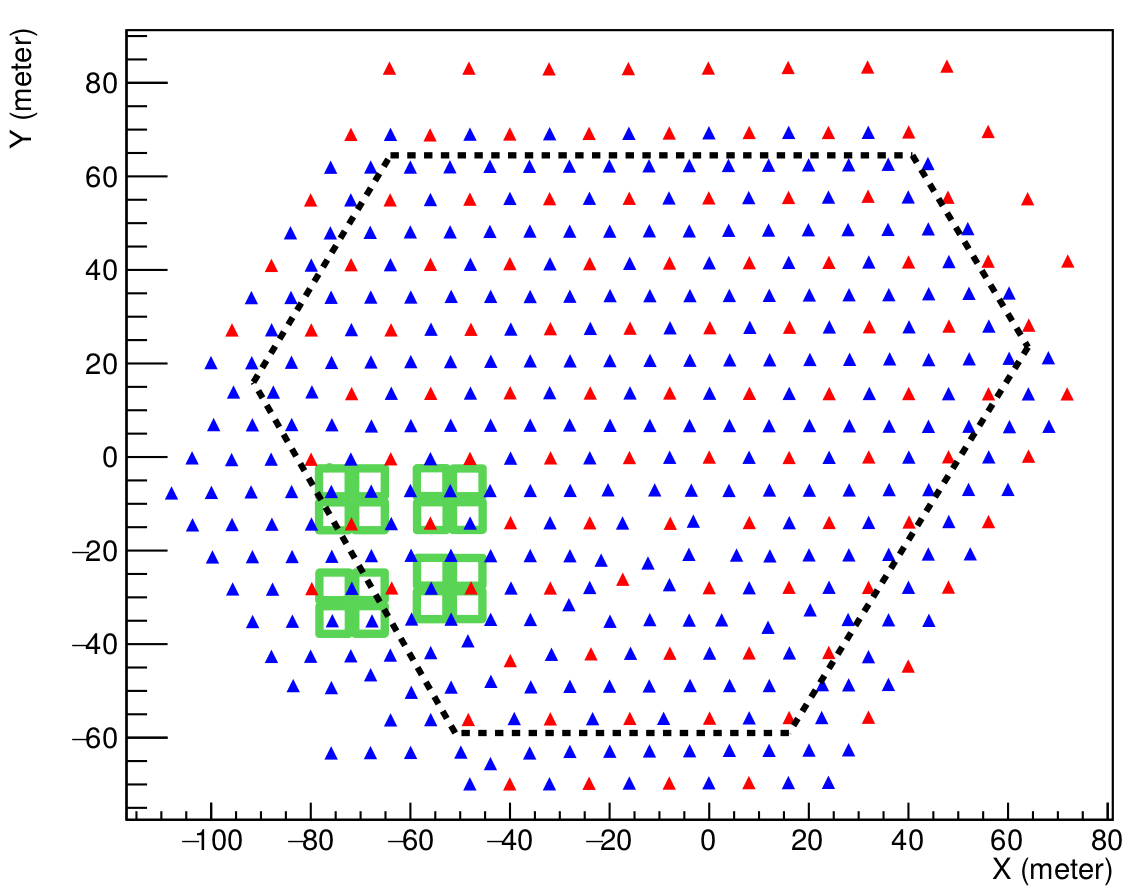
\includegraphics[width=0.9\linewidth, height=3cm]{array-map} 
\caption{Schematic of GRAPES-3 detector array}
\label{fig:array-map}
\end{subfigure}
\begin{subfigure}{0.245\textwidth}
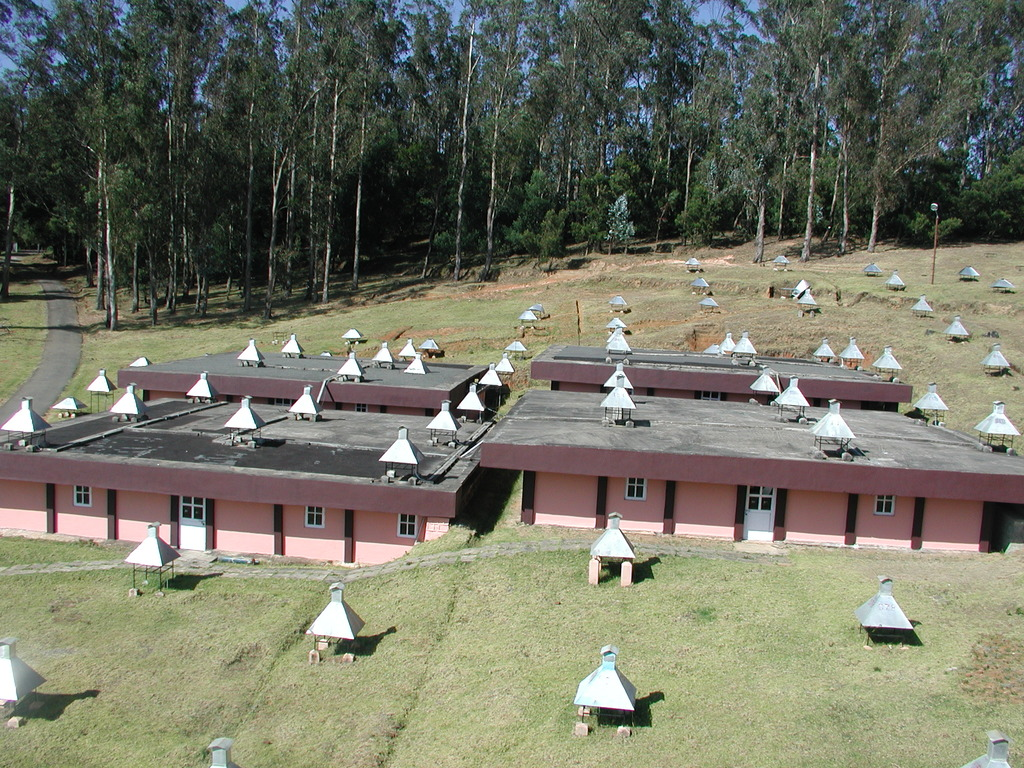
\includegraphics[width=0.9\linewidth, height=3cm]{detector} 
\caption{Scintillator detector and muon station}
\label{fig:detector}
\end{subfigure}
\begin{subfigure}{0.245\textwidth}
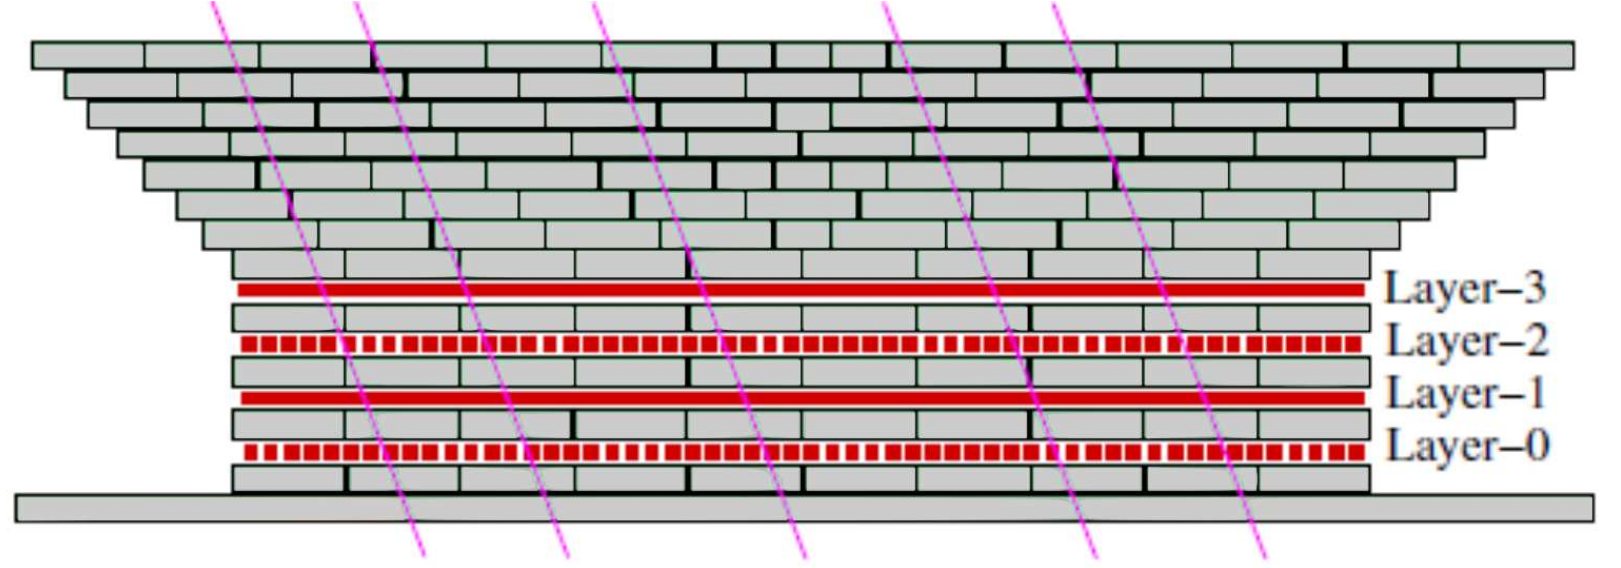
\includegraphics[width=0.9\linewidth, height = 3cm]{mu-station} 
\caption{Schematic of muon module}
\label{fig:mu-station}
\end{subfigure}
\begin{subfigure}{0.245\textwidth}
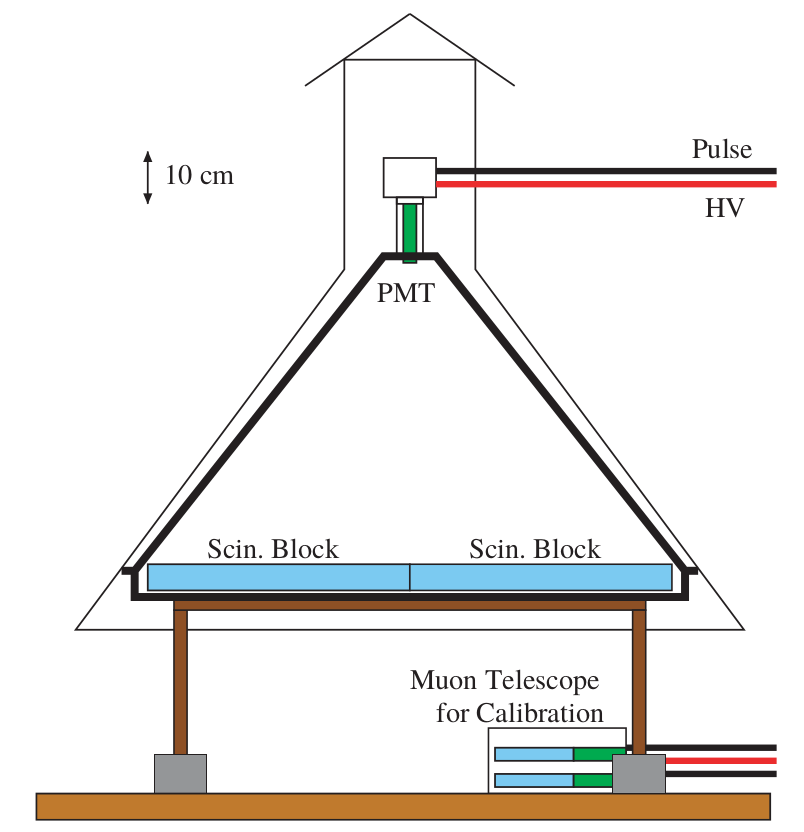
\includegraphics[width=0.9\linewidth, height = 3cm]{sc-detector}
\caption{Schematic of scintillator detector}
\label{fig:sc-detector}
\end{subfigure}
\caption{GRAPES-3 detector array}
\label{fig:g3array}
\end{figure}
 
The scintillator detectors (shown as filled triangles in Figure \ref{fig:array-map}) are spread over an area of $\sim$25,000 m$^2$. Each of the GRAPES-3 scintillator detector is 1 m$^2$ in area. The separation between two scintillator detectors is 8 m, which makes it one of the most dense array among the traditional EAS arrays. GRAPES-3 muon detector is comprised of 16 closely packed modules (shown as squares in Figure \ref{fig:array-map}). Each module contains 232 PRCs, placed in 4 layers, arranged in orthogonal directions. Each layer consists of 58 PRCs kept closely side by side. The effective area of each module is 35 m$^2$. This large area, muon detector has been designed for studies on the composition of primary cosmic rays and studies on cosmic sources of UHE $\gamma$-rays. 


\section{Simulation of monoenergetic showers}

For the treatment of low energy hadronic interactions, two low energy hadronic generators, namely FLUKA and GHEISHA, are commonly used. Table \ref{tab:fluka-gheisha} shows the difference in muon multiplicity produced by the two hadronic generators. Here, these were paired with SIBYLL 2.3c and QGSJETII-04 to treat high energy hadronic interactions. FLUKA combination gives higher muon multiplicity as compared to GHEISHA combination. In the earlier CORSIKA simulations, done for GRAPES-3 experiment, fluka was used as the low energy hadronic generator. So in this study also all the simulations were done using FLUKA as low energy hadronic generator. 

\begin{table}
\centering
\begin{tabular}{ | c | c | c | c |} 
\hline
Generator & Median & Sigma & Rel. S.D. (\%) \\ 
\hline
SIBYLL-GHEISHA &1161 & 273 & 23.5  \\ 
\hline
SIBYLL-FLUKA   & 1179 & 277 & 23.5  \\
\hline
QGSII-GHEISHA  & 1185 & 258 & 21.8  \\
\hline
QGSII-FLUKA  & 1200 & 250 & 20.8 \\
\hline
\end{tabular}
\caption{Comparison of muon  multiplicity distribution for a 100 TeV primary proton}
\label{tab:fluka-gheisha}
\end{table}

A comparison between the two post-LHC hadronic interaction generators was done to see the characteristics of the two generators. The comparison was done on the basis of muon content produced by the two generators. The PCRs were assumed to be composed of five species\cite{tanaka}, protons (H, A = 1), helium (He, A = 4), nitrogen (N, A = 14), aluminum (Al, A = 27) and iron (Fe, A = 56). Heavier nuclei N, Al and Fe were used to represent light (C,N,O), medium (Mg, Al, Si) and heavy (Mn, Fe, Co) masses in PCRs. For each primary, monoenergetic showers with zenith angle = 0 were simulated at energy: 10 TeV, 100 TeV, and 1000 TeV. Comparison of muon multiplicity was made: 1) between the two generators, 2) between different primaries for each generator.

Since the threshold energy of muon detector of GRAPES-3 experiment is 1(Sec($\theta$)) GeV ]\cite{hayashi} for muons incident on the detector with zenith angle $\theta$ (with coverage upto 45$^\circ$), in simulations also the muons with energy greater 1(Sec($\theta$)) GeV were counted. Table \ref{tab:muon_multiplicity} shows the variation of median muon multiplicity with changing primaries, primary energies, and with different generators. 

\begin{table}
\centering
%\begin{tabular}{ | p{1.5cm} | p{2cm} | p{1.5cm} | p{2cm} | p{1.5cm} |} 
\begin{tabular}{ | c | c | c | c | c | c |} 
\hline
& \multicolumn{2}{|c|}{\textbf{SIBYLL-FLUKA}} & \multicolumn{2}{|c|}{\textbf{QGSJETII-FLUKA}} & S vs Q \\
\hline
 & Median & \% Increase & Median & \% Increase & \% Increase \\
\hline 
\multicolumn{6}{|c|}{\textbf{10 TeV}} \\
\hline
H 	&	146	&	      & 150 &			& 2.7 \\
\hline
He 	&	174 &	19.2 &	182	&	21.33	&	4.6	\\
\hline
N 	& 	214 & 	46.6 &	227	&	51.33	&6.0	\\
\hline
Al 	& 	239 & 	63.7 &	254	&	69.33	&6.3	\\
\hline
Fe 	& 	259 & 	77.4 &	278	&	85.33	&7.3	\\
\hline
\multicolumn{6}{|c|}{\textbf{100 TeV}} \\
\hline
H & 1180 &  & 1200 & & 1.7 \\
\hline
He & 1340 & 13.6  & 1375 & 14.58	& 2.6\\
\hline
N & 1531 & 29.8 & 1577 & 31.42 	& 3.0\\
\hline
Al & 1659 & 40.6 & 1724 & 43.67 	& 3.9\\
\hline
Fe & 1845 & 56.4 & 1931 & 60.92	& 4.7\\
\hline
\multicolumn{6}{|c|}{\textbf{1000 TeV}} \\
\hline
H & 9393 &  & 9586 & & 2.1\\
\hline
N & 12132 & 29.2 & 12337 & 28.7 & 1.7\\
\hline
Fe & 13874 & 47.7 & 14284 & 49.0 & 3.0\\
\hline
\end{tabular}
\caption{Median muon multiplicity at 10 TeV, 100 TeV, and 1000 TeV. Column 3 and 5 show the percentage increase in muon multiplicity of different primaries w.r.t. H of respective generators. Column "S vs Q" shows the percentage increase in muon multiplicity in QGSJETII-FLUKA w.r.t. that of SIBYLL-FLUKA.\label{tab:muon_multiplicity}}
\end{table}

Table \ref{tab:muon_multiplicity} shows that QGSJETII-FLUKA gives slightly higher muon multiplicity as compared to SIBYLL-FLUKA and the difference increases with mass of primary. As the energy increases from 10 TeV to 1000 TeV, the difference in muon multiplicity of two generators decrease. Figure \ref{fig:sibyllmm} and Figure \ref{fig:qgsiimm} show the muon multiplicity distributions  at different primary energies.

\begin{figure}
\begin{subfigure}{0.32\textwidth}
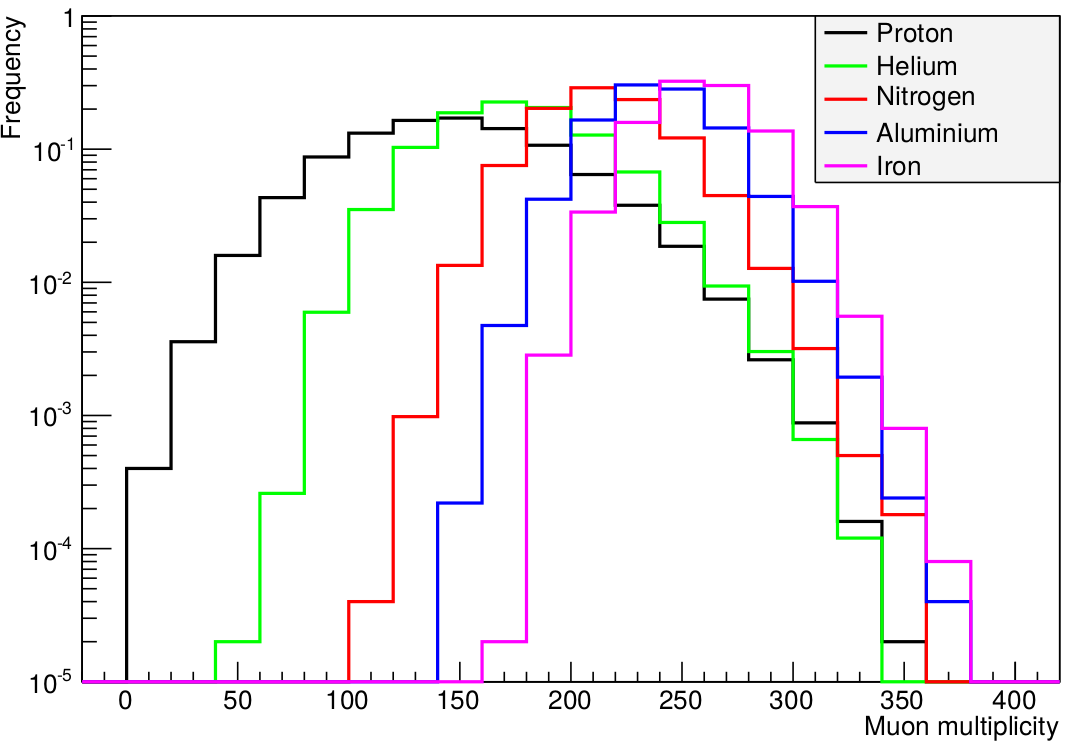
\includegraphics[width=0.9\linewidth, height=3cm]{sibyllmm10} 
\caption{10 TeV}
\label{fig:sibyllmm10}
\end{subfigure}
\begin{subfigure}{0.32\textwidth}
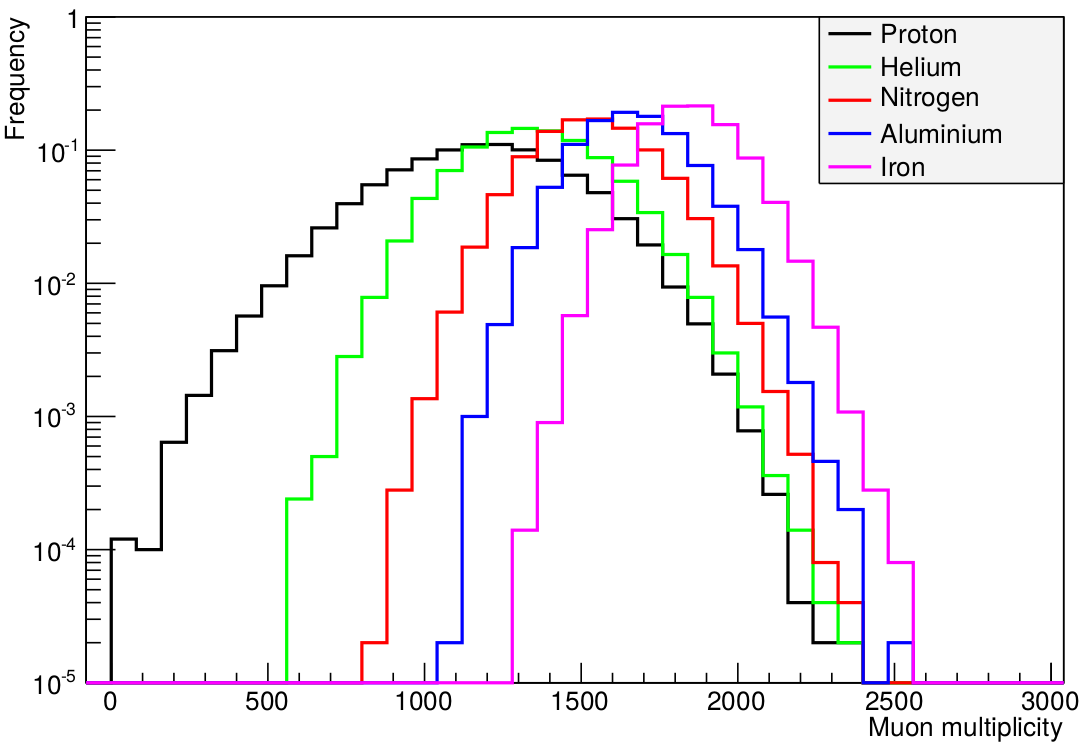
\includegraphics[width=0.9\linewidth, height=3cm]{sibyllmm100} 
\caption{100 TeV}
\label{fig:sibyllmm100}
\end{subfigure}
\begin{subfigure}{0.32\textwidth}
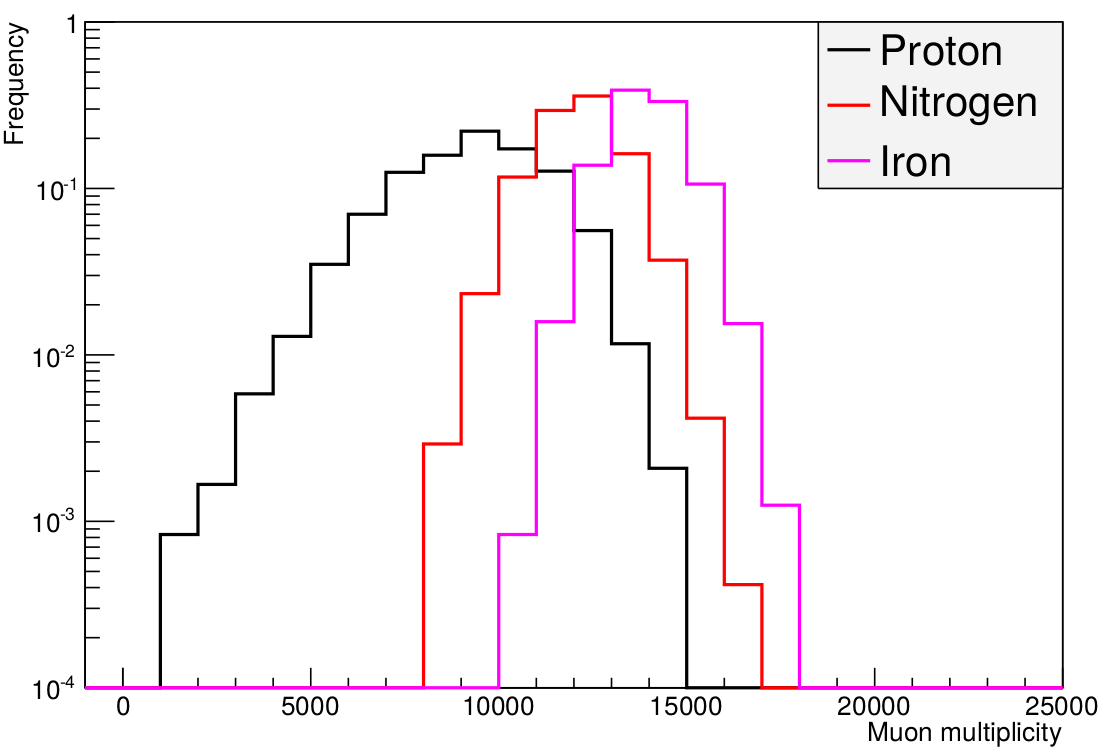
\includegraphics[width=0.9\linewidth, height = 3cm]{sibyllmm1000} 
\caption{1000 TeV}
\label{fig:sibyllmm1000}
\end{subfigure}
\caption{Muon multiplicity distribution for different primaries using SIBYLL-FLUKA}
\label{fig:sibyllmm}
\end{figure}
 

\begin{figure}
\begin{subfigure}{0.32\textwidth}
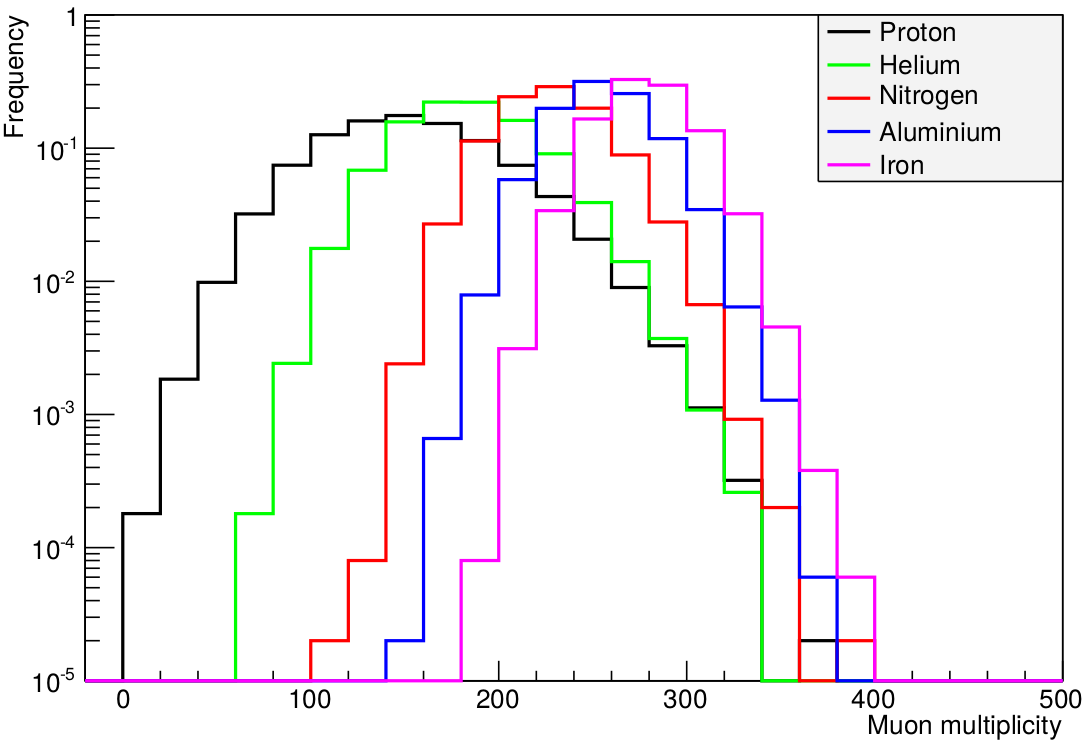
\includegraphics[width=0.9\linewidth, height=3cm]{qgsiimm10} 
\caption{10 TeV}
\label{fig:qgsiimm10}
\end{subfigure}
\begin{subfigure}{0.32\textwidth}
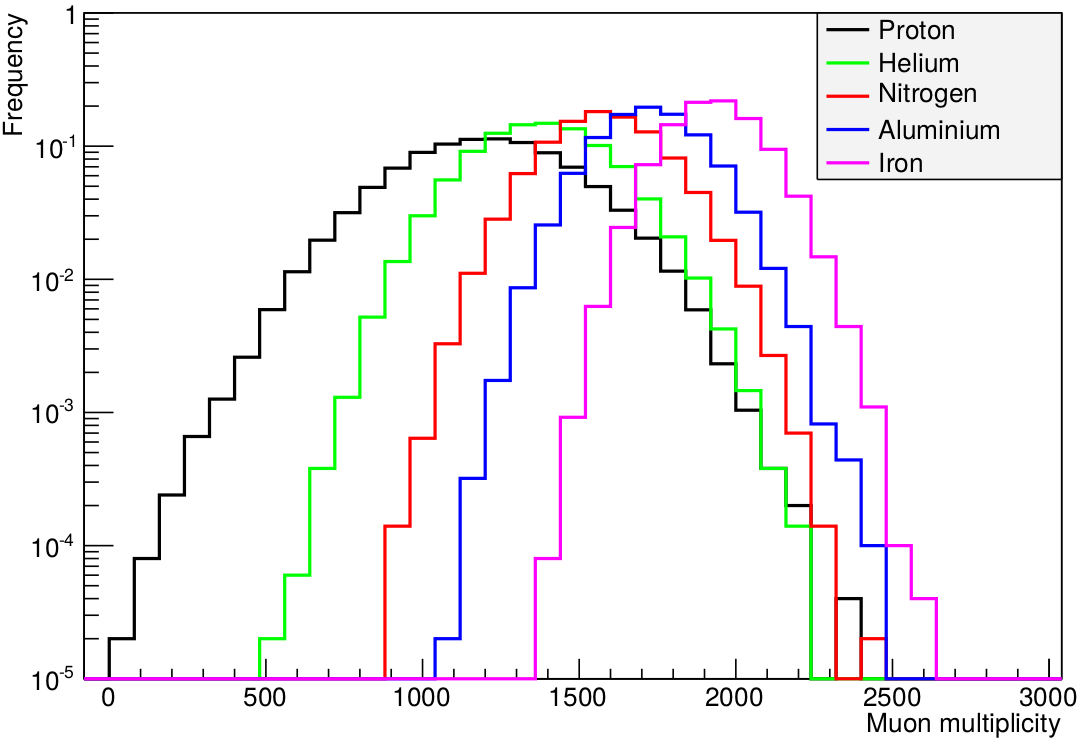
\includegraphics[width=0.9\linewidth, height=3cm]{qgsiimm100} 
\caption{100 TeV}
\label{fig:qgsiimm100}
\end{subfigure}
\begin{subfigure}{0.32\textwidth}
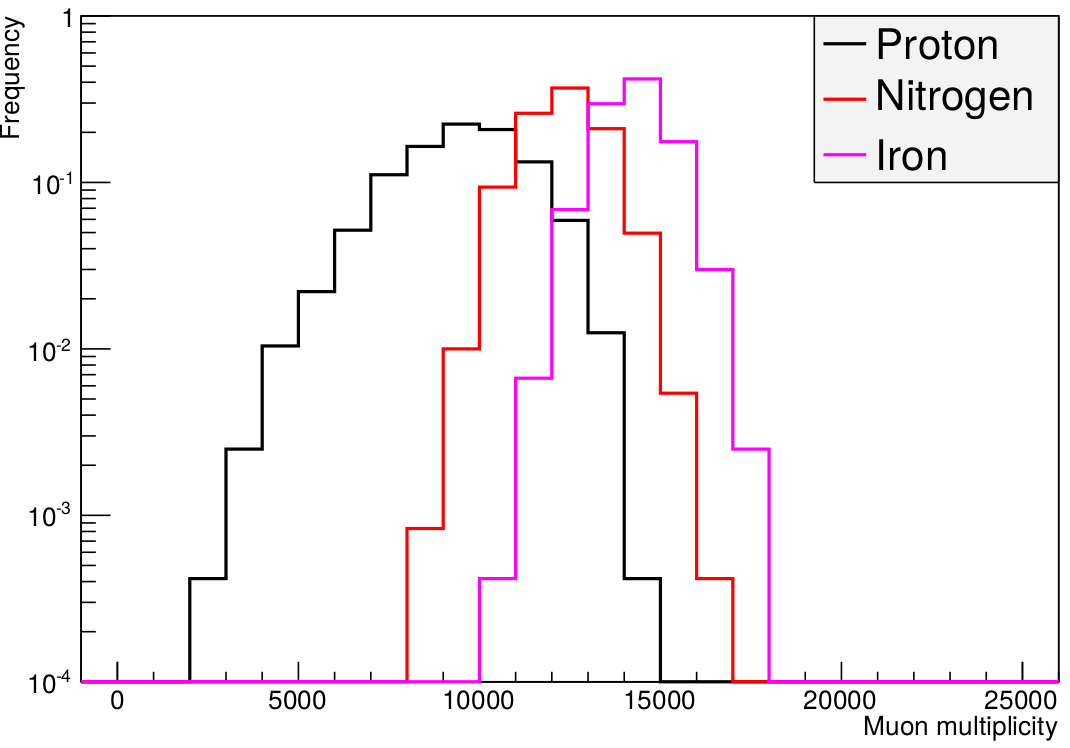
\includegraphics[width=0.9\linewidth, height = 3cm]{qgsiimm1000} 
\caption{1000 TeV}
\label{fig:qgsiimm1000}
\end{subfigure}
\caption{Muon multiplicity distribution for different primaries using QGSJETII-FLUKA}
\label{fig:qgsiimm}
\end{figure}


Monoenergeric proton induced showers with zenith angle = 0$^\circ$ were simulated using generators of CORSIKA-6.99, namely SIBYLL 2.1 and QGSJETII-03, at energies: 10 TeV, 100 TeV, and 1000 TeV. Table \ref{tab:muon_multiplicity_lhc} shows that the difference between median muon multiplicity of SIBYLL- and QGSJETII-FLUKA is more in pre-LHC as compared to post-LHC generators. In other words, post-LHC generators are expected to give relatively close results in shower analysis as compared to pre-LHC generators. Column 3 and column 5 of the Table \ref{tab:muon_multiplicity_lhc} show that the difference of median muon multiplicity between pre- and post-LHC generators is higher for more massive primaries. 


\begin{table}
\centering
\begin{tabular}{ | c | c | c | c | c | c |} 
\hline
& \multicolumn{2}{|c|}{\textbf{SIBYLL-FLUKA}} & \multicolumn{2}{|c|}{\textbf{QGSJETII-FLUKA}} & S vs Q \\
\hline
 & Median & \% Increase & Median & \% Increase & \% Increase \\
\hline 
\multicolumn{6}{|c|}{\textbf{10 TeV}} \\
\hline
Pre-LHC 	&	130	&	      & 142 &			& 9.2 \\
\hline
Post-LHC 	&	146	&	12.3      & 150 &	5.6		& 2.7 \\
\hline
\multicolumn{6}{|c|}{\textbf{100 TeV}} \\
\hline
Pre-LHC & 1006 &  & 1088 & & 8.2 \\
\hline
Post-LHC & 1180 & 17.3 & 1200 & 10.3 & 1.7 \\
\hline
\multicolumn{6}{|c|}{\textbf{1000 TeV}} \\
\hline
Pre-LHC & 7866 &  & 8327 & & 5.9\\
\hline
Post-LHC & 9393 & 19.4 & 9586 & 15.1 & 2.1\\
\hline
\end{tabular}
\caption{Median muon multiplicity at 10 TeV, 100 TeV, and 1000 TeV using pre-LHC and post-LHC generators. Column 3 and 5 represents the percentage increase in muon multiplicity of post-LHC hadronic generators w.r.t. that of pre-LHC hadronic generators. Column 6 represents the percentage increase in muon multiplicity of QGSJETII-FLUKA w.r.t. that of SIBYLL-FLUKA.\label{tab:muon_multiplicity_lhc}}
\end{table}

\begin{figure}
\begin{subfigure}{0.32\textwidth}
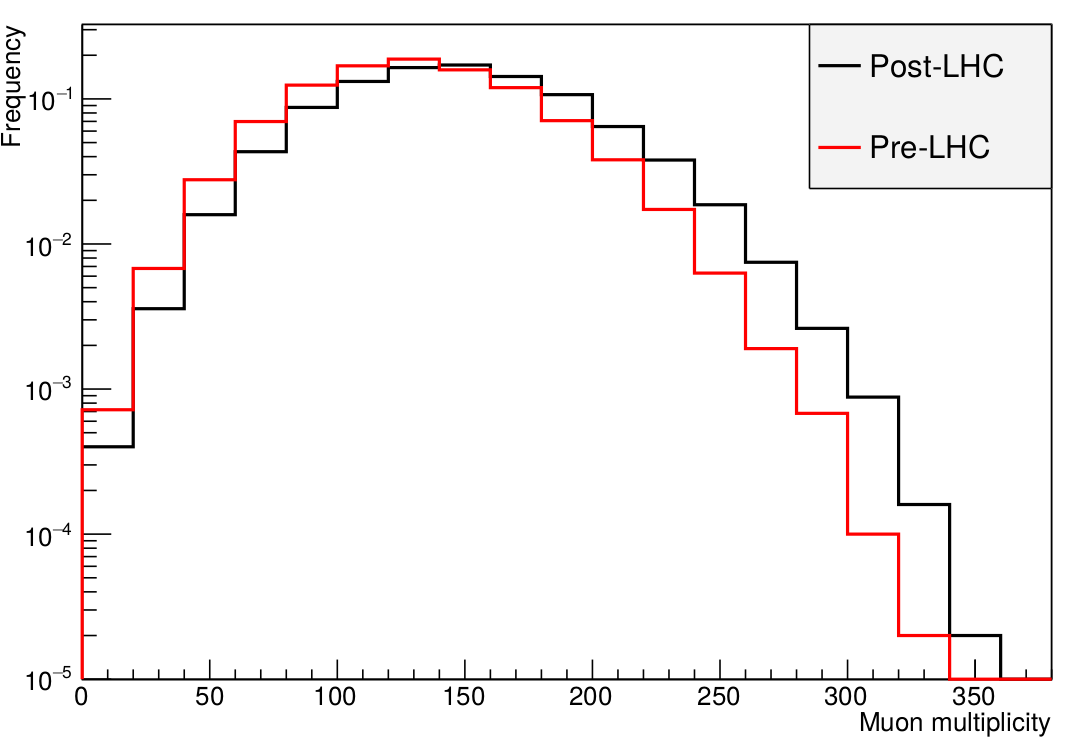
\includegraphics[width=0.9\linewidth, height=3cm]{sibyll-lhc-mm10} 
\caption{10 TeV}
\label{fig:sibyll-lhc-mm10}
\end{subfigure}
\begin{subfigure}{0.32\textwidth}
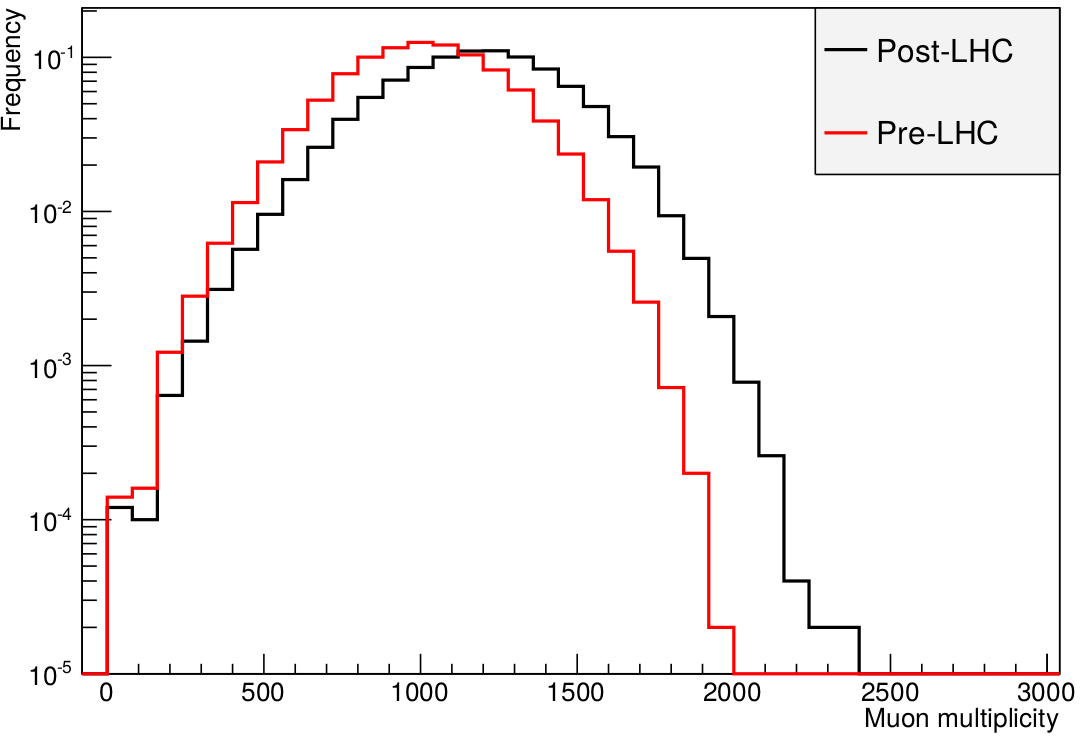
\includegraphics[width=0.9\linewidth, height=3cm]{sibyll-lhc-mm100} 
\caption{100 TeV}
\label{fig:sibyll-lhc-mm100}
\end{subfigure}
\begin{subfigure}{0.32\textwidth}
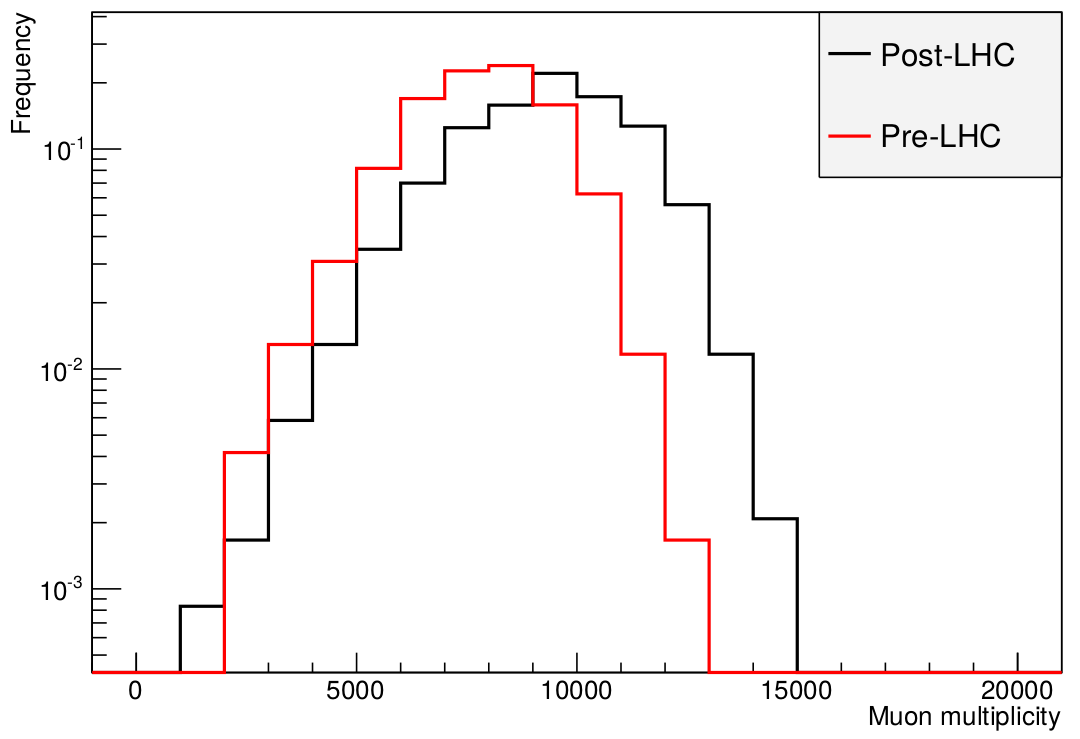
\includegraphics[width=0.9\linewidth, height = 3cm]{sibyll-lhc-mm1000} 
\caption{1000 TeV}
\label{fig:sibyll-lhc-mm1000}
\end{subfigure}
\caption{Muon multiplicity distribution of pre- and post-LHC hadronic generators (SIBYLL-FLUKA)}
\label{fig:lhc_multiplicity_sibyll}
\end{figure}



\begin{figure}
\begin{subfigure}{0.32\textwidth}
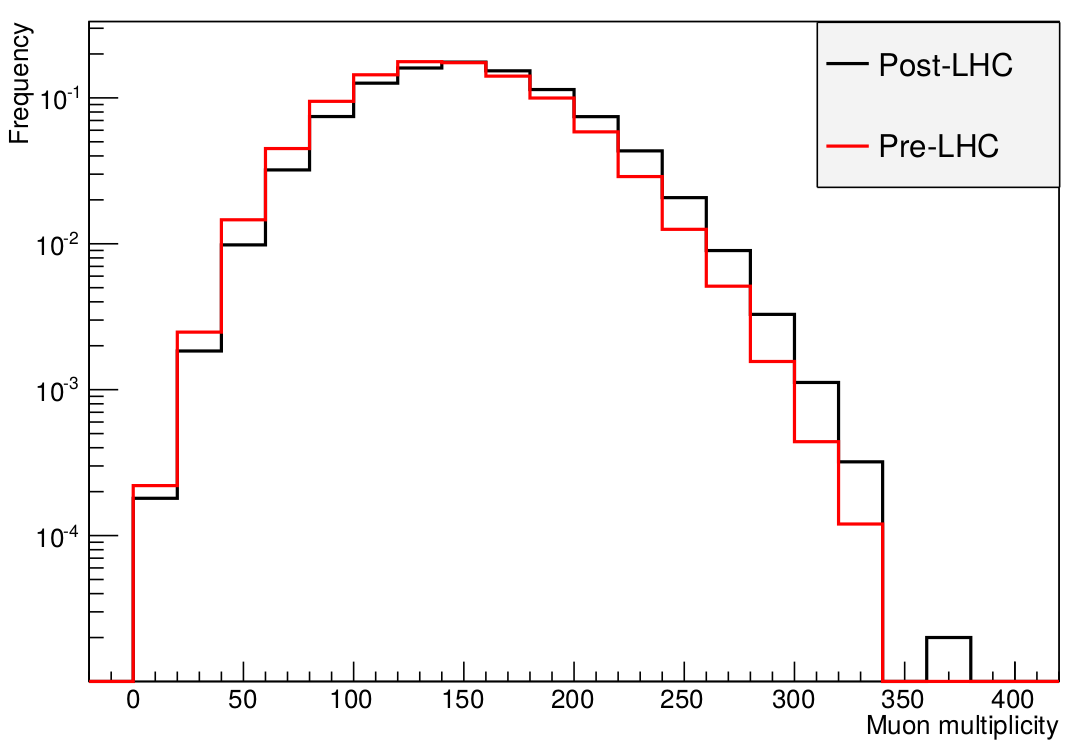
\includegraphics[width=0.9\linewidth, height=3cm]{qgsii-lhc-mm10} 
\caption{10 TeV}
\label{fig:qgsii-lhc-mm10}
\end{subfigure}
\begin{subfigure}{0.32\textwidth}
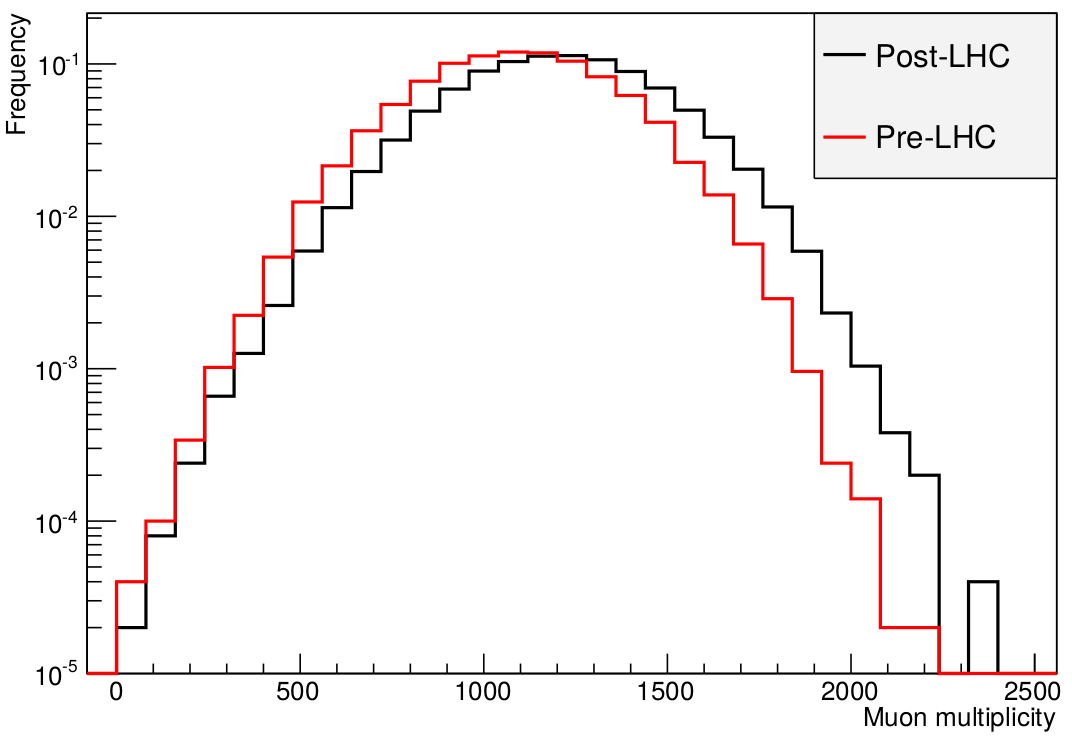
\includegraphics[width=0.9\linewidth, height=3cm]{qgsii-lhc-mm100} 
\caption{100 TeV}
\label{fig:qgsii-lhc-mm100}
\end{subfigure}
\begin{subfigure}{0.32\textwidth}
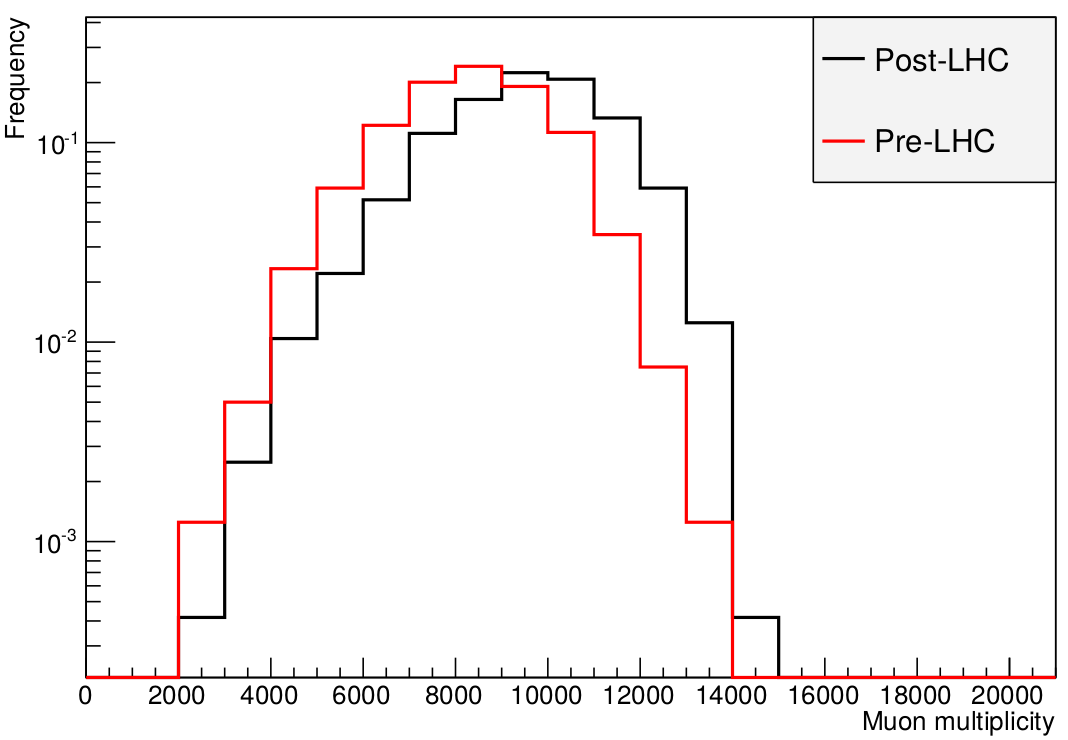
\includegraphics[width=0.9\linewidth, height = 3cm]{qgsii-lhc-mm1000} 
\caption{1000 TeV}
\label{fig:qgsii-lhc-mm1000}
\end{subfigure}
\caption{Muon multiplicity distribution of Pre- and Post-LHC hadronic generators (QGSJETII-FLUKA)}
\label{fig:lhc_multiplicity_qgsii}
\end{figure}

\section{Comparison of simulations results with GRAPES-3 data}
Study of monoenergetic showers was done to see the behaviour of different generators for different primary energies and primary types. For comparison with detector data, the pre-existing shower data was used which was generated using SIBYLL-2.1 (CORSIKA-7.41). The data was generated for the energy range of 1 TeV to 3000 TeV, in 15 logarithmic energy bins of bin width = 0.2. 999 files were generated in each energy bin with energy cuts of 50 MeV, 10 MeV, 1MeV, and 1MeV for hadrons, muons, electrons, and photons respectively. During the analysis of data for this study, events from bin 10 - bin 15 were used. There were 999 files for each energy bin and each file had 10 showers. Each shower was used 10 times, with it's core randomized, to increase the statistics. The spectrum was produced using this data with spectral index of -2.7. The number of events used from each bin are shown in Table \ref{tab:binning}. 

\begin{table}[h]
\centering
\begin{tabular}{ | c | c | c |} 
\hline
Bin No. & Energy Range (TeV) & No. of events analysed  \\ 
\hline
10 & 63.10 - 100 & 99900  \\ 
\hline
11 & 100 - 158.49 & 45700  \\
\hline
12 & 158.49 - 251.19 & 20900 \\
\hline
13 & 251.19 - 398.11 & 9500 \\
\hline
14 & 398.11 - 630.96 & 4400 \\
\hline
15 & 630.96 -1000 & 2000 \\
\hline
\end{tabular}
\caption{Number of events analysed from each energy bin}
\label{tab:binning}
\end{table}

The core of each shower was randomized in a circular radius  = 150 m around the array center. Then only those showers were processed which fell inside the fiducial area of array (shown by dashed line in Figure \ref{fig:array-map}), and satisfied trigger0 and trigger1 condition of detector array\cite{gupta}. In this work, analysis code used to analyze the simulated showers was improved. The code now can detect the muons hitting individual layers of the muon detector. If muon hits the following layers: layer 0 and layer 2 , or layer 1 and layer 3, or all layers , the muon hit is considered. Only those muons were counted which had kinetic energy greater than 1(Sec($\theta$)) GeV on the muon detector surface. Then, the muon multiplicity spectrum was created for shower size (N$_e$) varying from 10$^3$ to 10$^7$ with bin width = 10$^{0.5}$. 

GRAPES-3 data of year 2014 (3 January to 30 December) was analysed and MMDs were created for each size bin. This spectrum was compared to that of GRAPES-3 data, for each bin. Figure \ref{fig:mmbin} shows the normalized MMDs for three differential shower size bins. From previous observations, it's known that the shower size 10$^{4.0}$ corresponds to  primary energy $\sim$50 TeV. and shower size 10$^{5.5}$ corresponds to primary energy $\sim$1000 TeV. Hence, MMD of only these shower size bins are compared. 

For higher muon multiplicities in either of the three plots, the statistics of simulation data are not very good. This was expected because the muon multiplicity of experimental data also has contribution from other type of primaries. As shown by Figure \ref{fig:sibyllmm}m the lower values of muon multiplicity are dominated by proton. Therefore, in Figure \ref{fig:mmbin}, we compare the region of low muon multiplicities i.e. region around the peak. 

The position of the peak of simulation data in Figure \ref{fig:mmbin2} matches to that of GRAPES-3 data. For higher size bins, the position peaks of the two distributions do not match but the difference is not very large. For higher shower size bins, the distributions from poor statistics. This is expected to improve with the analysis of post-LHC spectrum data because as was shown earlier, SIBYLL-2.3c produces upto $\sim$ 19 \% more muons w.r.t to SIBYLL-2.1. 

\begin{figure}[h]
\begin{subfigure}{0.32\textwidth}
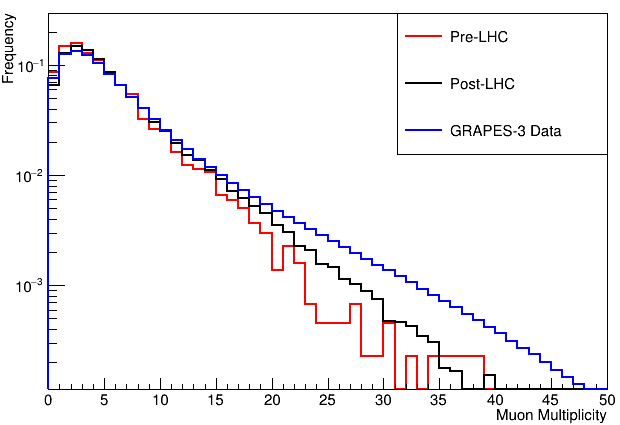
\includegraphics[width=0.9\linewidth, height=3cm]{mmbin2} 
\caption{Shower size - 10$^{4.0}$ to 10$^{4.5}$}
\label{fig:mmbin2}
\end{subfigure}
\begin{subfigure}{0.32\textwidth}
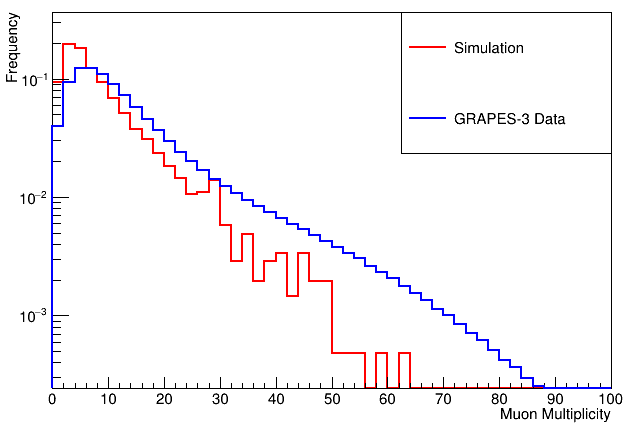
\includegraphics[width=0.9\linewidth, height=3cm]{mmbin3} 
\caption{Shower size - 10$^{4.5}$ to 10$^{5.0}$}
\label{fig:mmbin3}
\end{subfigure}
\begin{subfigure}{0.32\textwidth}
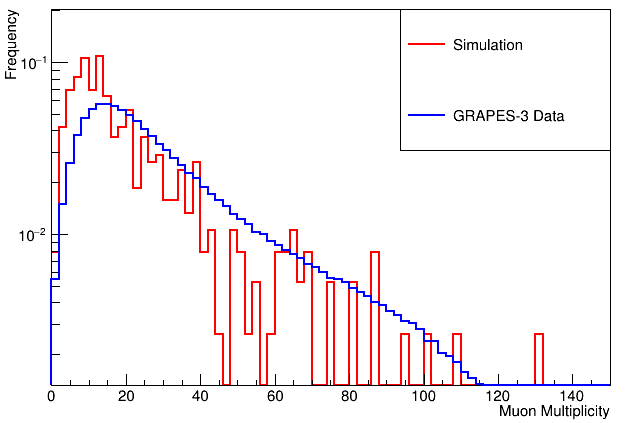
\includegraphics[width=0.9\linewidth, height = 3cm]{mmbin4} 
\caption{Shower size - 10$^{5.0}$ to 10$^{5.5}$}
\label{fig:mmbin4}
\end{subfigure}
\caption{Comparison of MMD between pre-LHC simulation data (SIBYLL-2.1) with GRAPES-3 data (3 January, 2014 to 30 December 2014)}
\label{fig:mmbin}
\end{figure}

\section{Summary}

Two hadronic interaction generators from CORSIKA 7.69 simulaton package: SIBYLL-2.3c and QGSJETII-04, were compared on the basis of muon content produced by each generator. Low energy hadronic interactions were treated by FLUKA-2011. MMDs of monoenenergetic showers with zenith angle = 0$^\circ$, induced by H, He, N, Al, and Fe at energies$-$10 TeV, 100 TeV, and 1000 TeV were compared. Muons produced by QGSJETII-FLUKA were found to be 1.7\% to 7.3\% higher than  that of SIBYLL-FLUKA. The difference between muon content of the two generators decreased with increasing primary energy. For each primary energy, the difference between the two generators increased as the primary became more massive.

MMDs of monoenergetic proton initiated showers simulated using post-LHC generators (SIBYLL 2.3c and QGSJETII-04) were  also compared with that of pre-LHC generators (SIBYLL-2.1 and QGSJETII-03 of CORSIKA-6.99). Proton iniated showers were simulated at energies: 10 TeV, 100 TeV, and 1000 TeV using above-mentioned post-LHC and pre-LHC generators. SIBYLL 2.3c produced 12.3\% to 19.4\% higher than that of SIBYLL-2.1. QGSJETII-03 produced 5.6\% to 15.1\% more muons than that of SIBYLL-2.1. Among pre-LHC generators, QGSJETII-03 produced 5.9\% to 9.2\% more muons than that of SIBYLL-2.1. Among post-LHC generators, QGSJETII-04 produced 1.7\% to 2.7\% more muons than that of SIBYLL-2.3c. Thus, the difference between muon content produced by QGSJETII and SIBYLL has decreased after tuning of the generator parameters to the LHC data.

Proton initiated showers with primary energy $63.1\times10^{12}$ eV $ < $ E $<1000\times10^{12}$ eV, and zenith angle $0^\circ<\theta<25^\circ$ were analysed. The muon multiplicity distribution for differential shower size bins was compared with data recorded by the GRAPES-3 detector in the year 2014 (3 January to 30 December). The data close to the peaks, which was most relevant for protons' contribution to GRAPES-3 data, of the distribution matched well with that of GRAPES-3 data. The difference near the peak regions increased with increasing shower size because of poor statistics of simulated data. This distribution of simulated data is expected to improve with the analysis of post-LHC (SIBYLL 2.3c) spectrum data. 

\section{Acknowledgments}
I thank Dr. Pravata K. Mohanty for his invaluable guidance through out this work. I thank my GRAPES-3 group members: Mr. B. Hari Haran, Mr. Fahim Varsi, Mr. Diptiranjan Pattanaik, Ms. Medha Chakraborty, and Mr. Meeran Zuberi for helping me out whenever I faced problems with the data analysis. I thank Mr. Samuel D. Morris for providing technical help to keep my work going, as he was handling the server I was working on.  

\begin{thebibliography}{9}

\bibitem{tanaka} H.Tanaka et al., J. Phys. G: Nucl. part. Phys. 39 (2012) 025201 (16pp) 

\bibitem{gupta} S.K. Gupta et. al, Nucl. Instr. and Meth. A 540 (2005) 311-323.
 
\bibitem{hayashi} Y. Hayashi et.al, "A large area muon tracking detector for ultra-high energy cosmic ray astrophysics—the GRAPES-3 experiment", url: https://doi.org/10.1016/j.nima.2005.02.020.

\bibitem{anuj} Anuj Chandra, "A Study of High-Energy Cosmic Ray Showers by Extending the Dynamic Range of Scintillator Detectors in GRAPES-3 Experiment", PhD Thesis.

\bibitem{mthesis} Stephan Runderkamp, url: https://esc.fnwi.uva.nl/thesis/centraal/files/f512727007.pdf

\end{thebibliography}




\end{document}

